\section{Generative Models}

\subsection{Energy-Based Models}

\subsubsection{Restricted Boltzmann Machines (RBMs)}

\paragraph{Pseudolikelihood}

Computing the log likelihood for MLE on a RBM requires summing over $2^{\lvert v' \rvert + \lvert h' \rvert}$
combinations of binary visible and hidden variables $v' \in \{0, 1\}, h' \in \{0, 1\}$.

\vspace{-10pt}

\begin{equation}
    \hspace{-7.5pt}
    \theta^*_\text{MLE}
    = \arg\max_\theta{P(v \mid \theta)}
    = \arg\max_\theta{\sum_h{P(v, h \mid \theta)}}
    = \arg\max_\theta{\mathcal{L}(\theta)}
    \propto \arg\max_\theta{\log{\mathcal{L}(\theta)}}
\end{equation}

\begin{equation}
    \log{\mathcal{L}(\theta)}
    = \log{\frac{1}{Z(\theta)}\sum_h{e^{-E(v, h; \theta)}}}
    = \log{\sum_h{e^{-E(v, h; \theta)}}} - \log{\sum_{v', h'}{e^{-E(v', h'; \theta)}}}
\end{equation}

The (log) pseudolikelihood \citep{Goodfellowetal2016} approximates the (log) likelihood as the
product of visible states $v'_i$'s conditional probabilities given all other visible states $v_{j \neq i}$.

\begin{equation}
    \log{\mathcal{L}(\theta)}
    = \log{P(v \mid \theta)}
    = \log{\prod_i{P(v_i \mid v_{j \neq i}; \theta)}}
    = \sum_i{\log{P(v_i \mid v_{j \neq i}; \theta)}}
\end{equation}

Pseudolikelihood (PL) is an \textit{approximation} technique that makes the training faster and \textit{tractable} on larger networks.
Having said that, training based on an approximation technique will not be as precise as an exact method.
The quality of learned representations will depend on the extent to which PL is able to approximate the true likelihood.

Another popular approximation used for training RBMs is Contrastive Divergence.
CD uses sampling (namely Gibbs sampling), and as such is \textit{stochastic};
PL is \textit{deterministic}.

\paragraph{Hyperparameter Tuning}

Increasing the number of \textit{components} or hidden units improves performance.
With 100 components it is possible to learn more patterns than with 50 or 10.
But there are signs of diminishing returns at this point.
Moreover, it becomes computationally heavier and much slower
(despite calculating the \textit{pseudo}likelihood).

A \textit{learning rate} of 0.01 is appropriate for 100 components. For 10, $\approx 0.1$ is better.\footnote{
    As in general, the trade-off is between training speed, risk of stagnation or overshooting minima.
}

Increasing the number of \textit{iterations} from 10 to 20 or 30 yields marginally better pseudolikelihood values.
Given that the training also takes 2 or 3 times as long,
more than 20 iterations may not be worth it unless maximising pseudolikelihood is paramount.

\begin{table}[h]
\centering
\begin{tabular}{|c|c|c|c|c|}
    \hline
    No. of components & Learning rate & No. of iterations & PL & Avg. time / it. \\
    \hline
    10 & 0.01 & 10 & -187.61 & 4.1s \\
    \hline
    50 & 0.01 & 10 & -98.75 & 5.9s \\
    \hline
    100 & 0.01 & 10 & -79.74 & 13.2s \\
    \hline
    100 & 0.001 & 10 & -109.78 & 13.7s \\
    \hline
    100 & 0.05 & 10 & -87.49 & 13.6s \\
    \hline
    100 & 0.1 & 10 & -96.93 & 13.5s \\
    \hline
    100 & 0.01 & 20 & -76.54 & 13.2s \\
    \hline
    100 & 0.01 & 30 & -75.07 & 13.2s \\
    \hline
\end{tabular}
\caption{Training a Bernoulli RBM on MNIST with different hyperparameters}
\label{tab:rbm-training}
\end{table}

A model with more hidden units can learn a more varied set of latent features.
A model with fewer hidden units learns fewer, more general features.
In unsupervised learning there is no overfitting but since a very large model has a lot of capacity it
could memorise data and may have reduced ability to generate diverse or novel samples.
A good model should produce a distribution that manages to capture the training distribution
and to reliably generate similar outputs, without explicitly memorising training inputs.

\paragraph{Gibbs Sampling from Model}

Gibbs sampling from the trained model with test data demonstrates how it can
generate variations of the test data based on the learned data distribution.
It is a Markov Chain Monte Carlo (MCMC) technique to draw from the joint distribution by alternating between $h \sim P(h \mid v)$ and $v \sim P(v \mid h)$
s.t. after some number of steps the sample should resemble the learned model distribution, $v \sim P(v)$.

Taking only one Gibbs sampling step generates data that is minimally different from the test data.
The more Gibbs sampling steps are performed, the more representative the generated images become of the distribution of representations learned by the model.

\paragraph{Image Reconstruction}

Reconstructions are not perfect but with 1 to 5 Gibbs steps the model is able to reconstruct images with up to 15 rows quite well.
With more Gibbs steps, e.g. 100, the reconstruction for close to half of the digits diverges and looks quite different; this is to be expected.
With 20 or more rows removed in the original image, the digit in it is not recognisable anymore, and the model is not able to reconstruct it.
A 2, e.g., is most difficult to reconstruct if the lower rows of the image are removed.

\subsubsection{Deep Boltzmann Machines (DBMs)}

\paragraph{Filters / Interconnection Weights}

A Deep Boltzmann Machine (DBM) consists of multiple layers of hidden units, where each layer is connected only to the adjacent layers (i.e., no intra-layer or skip connections).
The features learned in the first hidden layer are simple patterns like edges or shapes, similar to those learned in the RBM.
The second hidden layer captures more complex combinations of features from the first layer.
Multiple layers enable learning more complex, hierarchical representations.

\begin{figure}[h!]
    \begin{minipage}[t]{0.19\textwidth}
        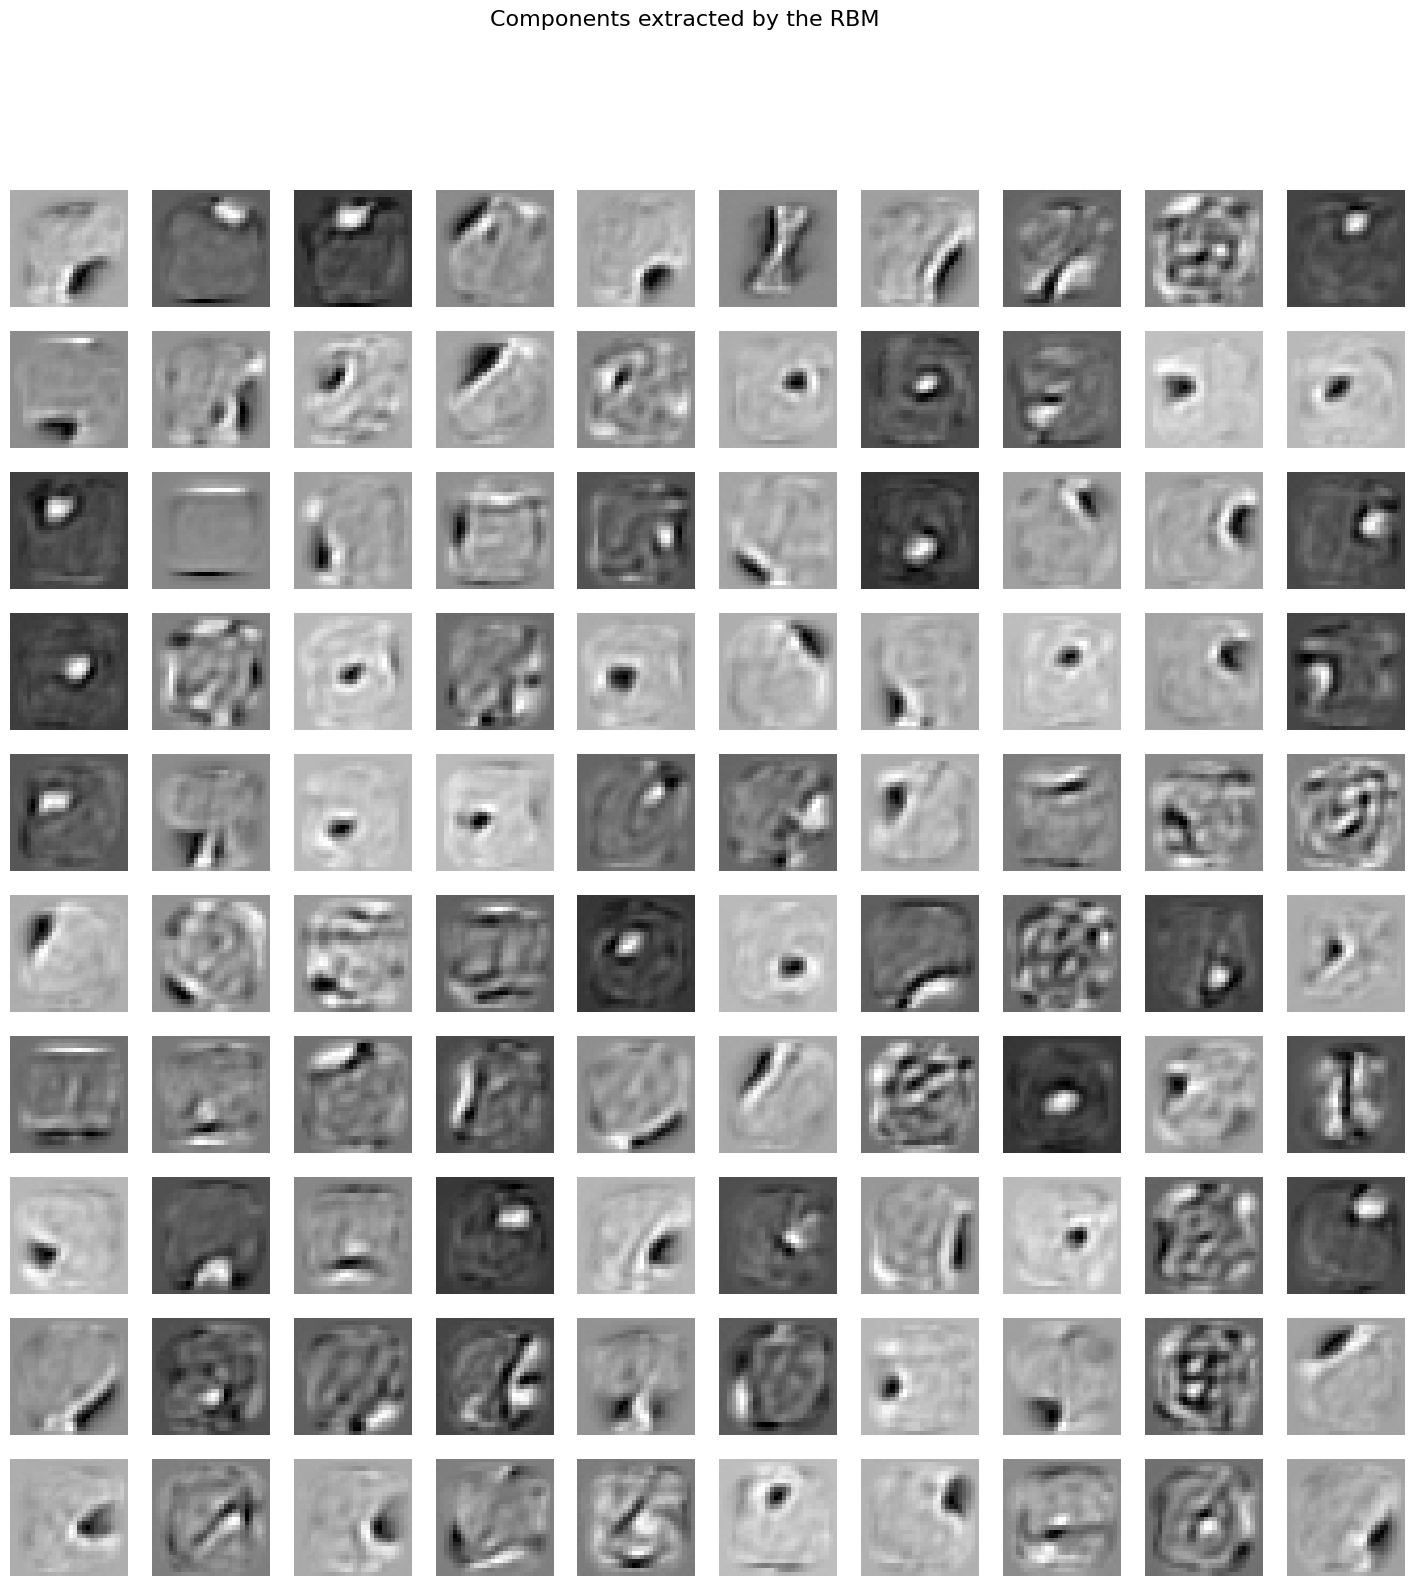
\includegraphics[width=\textwidth]{figures/rbm-features.png}
    \end{minipage}
    \hfill
    \begin{minipage}[t]{0.19\textwidth}
        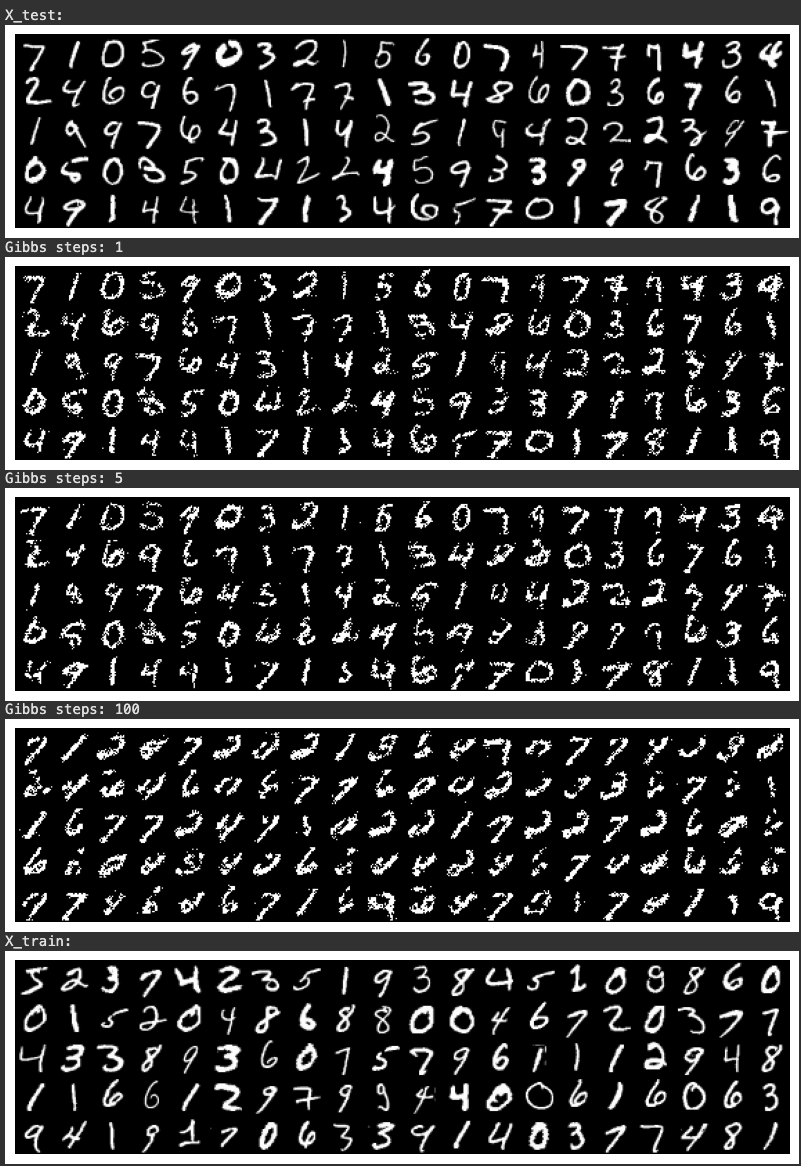
\includegraphics[width=\textwidth]{figures/rbm-generation.png}
    \end{minipage}
    \hfill
    \begin{minipage}[t]{0.19\textwidth}
        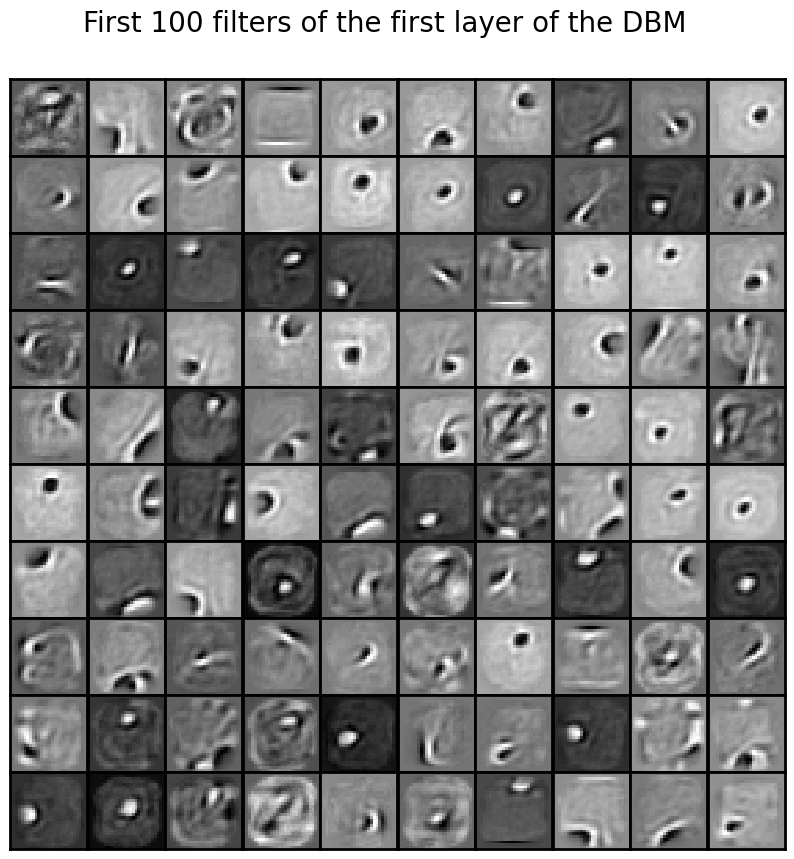
\includegraphics[width=\textwidth]{figures/dbm-layer1-features.png}
    \end{minipage}
    \hfill
    \begin{minipage}[t]{0.19\textwidth}
        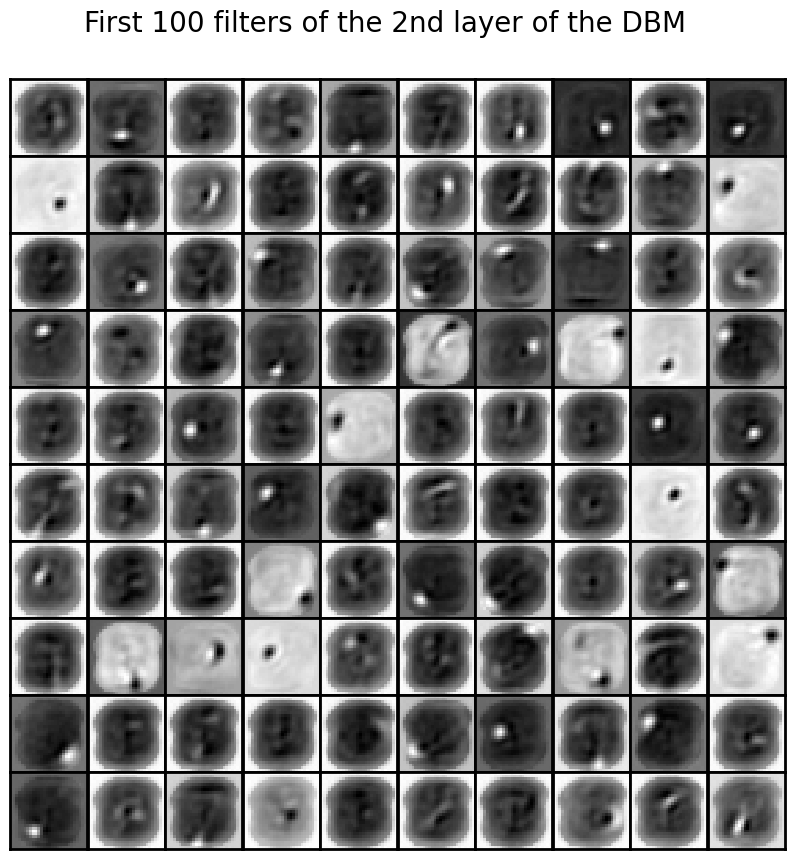
\includegraphics[width=\textwidth]{figures/dbm-layer2-features.png}
    \end{minipage}
    \hfill
    \begin{minipage}[t]{0.19\textwidth}
        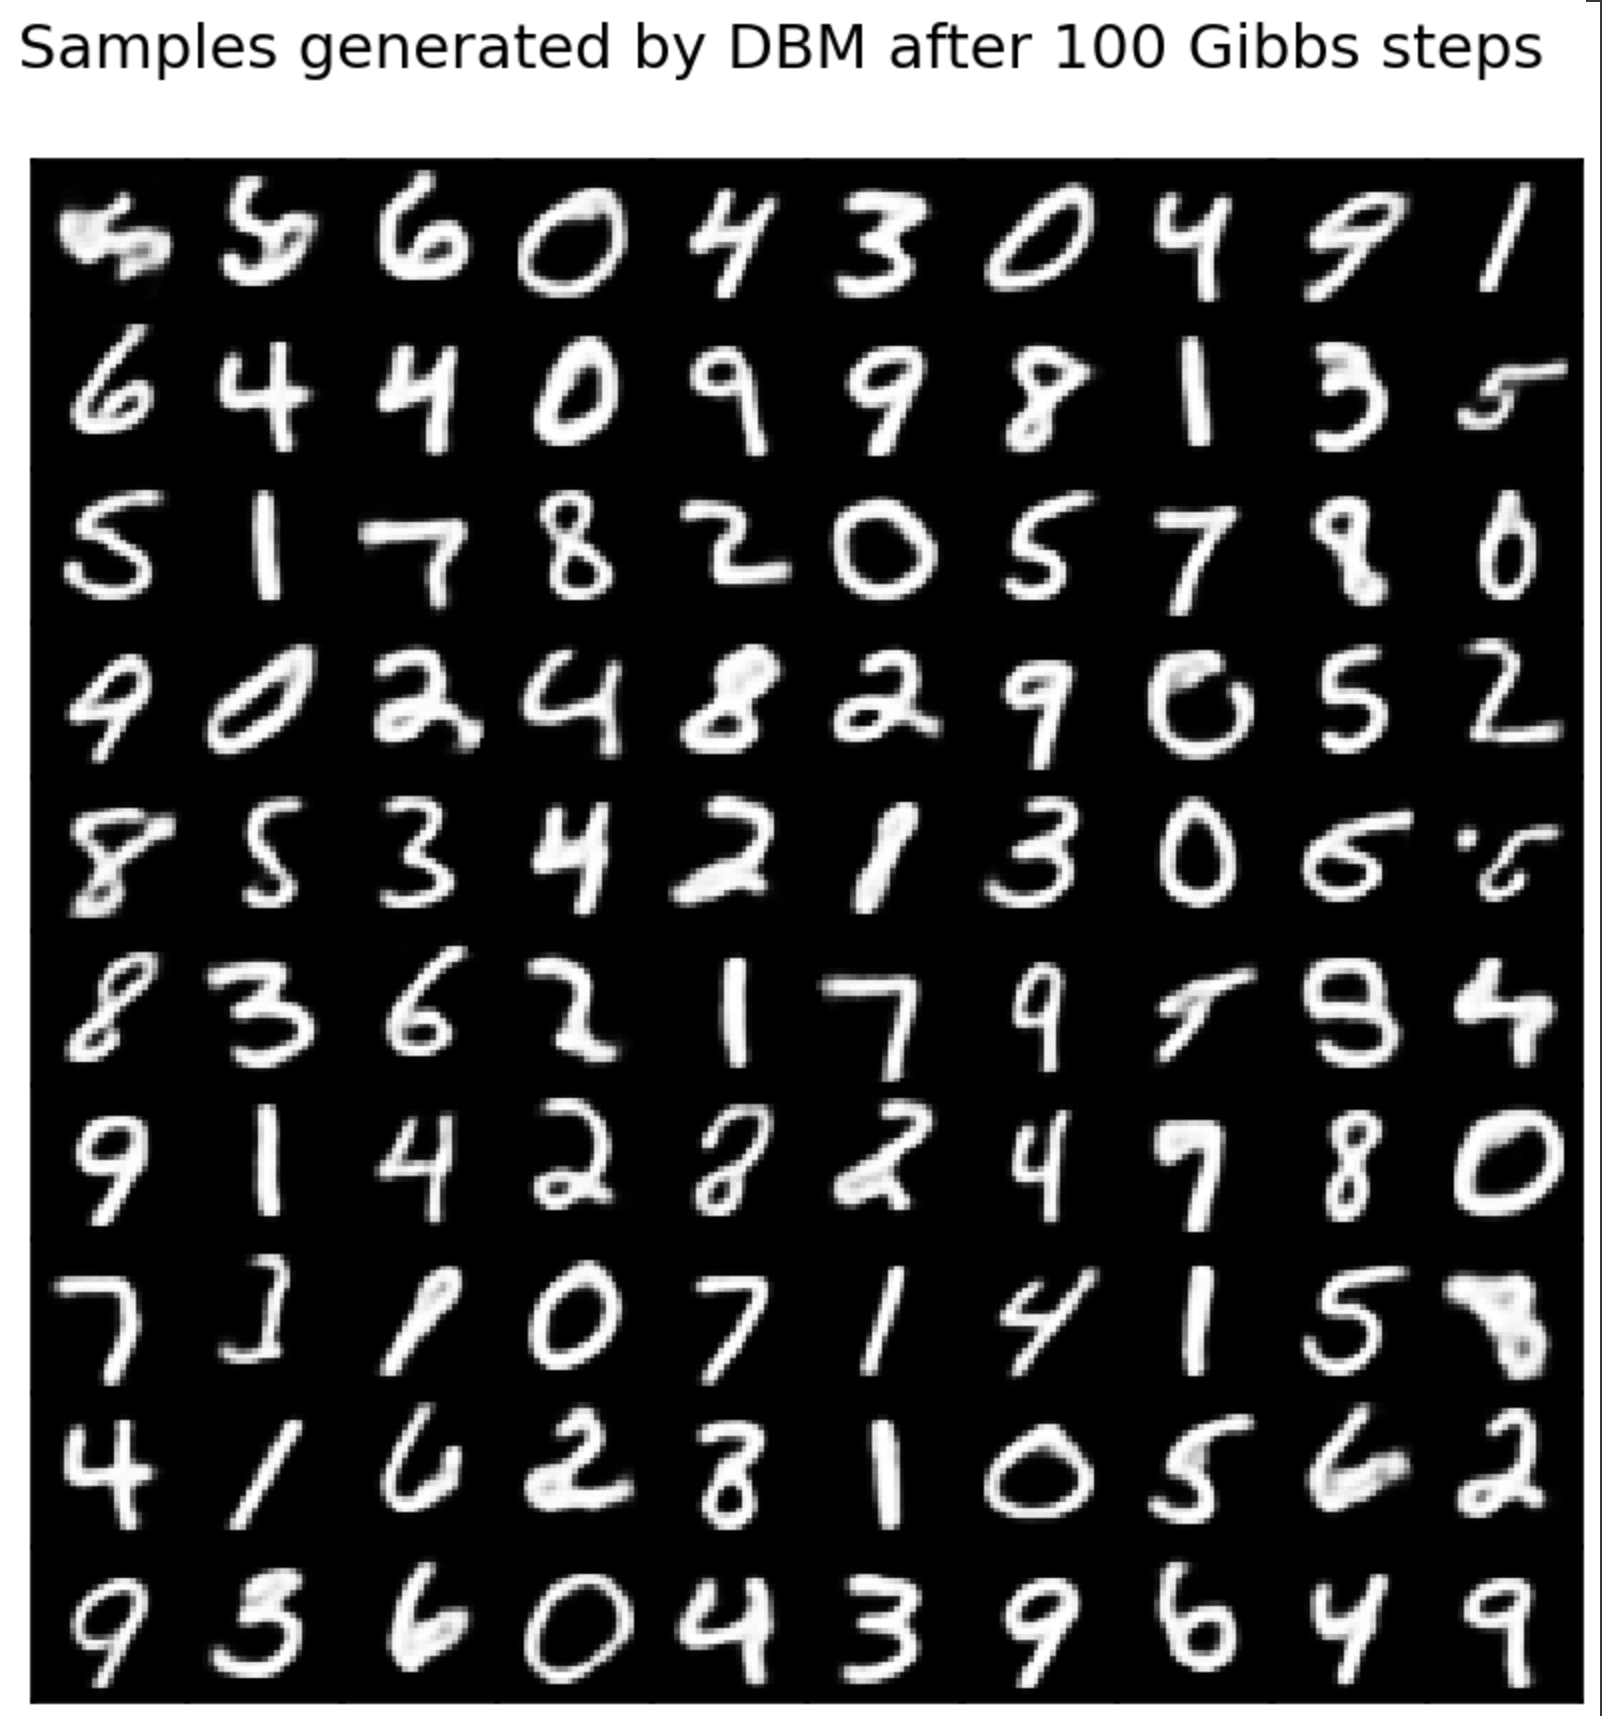
\includegraphics[width=\textwidth]{figures/dbm-generation.png}
    \end{minipage}
    \caption{RBM vs. DBM comparison: learned features and sampled images}
    \label{fig:rbm-dbm-features-generation}
\end{figure}
\vspace{-10pt}

\paragraph{Model Evaluation}

There are still some outputs that do not look like a digit.
But overall the quality of the samples generated by the DBM is higher and they are more realistic.
The distribution is more random and a greater variety of different digits is generated.
The multiple layers enable the DBM to learn more high-level features and therefore to generalise better in terms of generation and reconstruction of images.

\newpage

\subsection{Generative Adversarial Networks (GANs)}

\subsubsection{Loss Functions}

Generative Adversarial Networks (GANs) are set up as a zero-sum game between
a Generator network (G) which generates samples and receives payoff $-v(\theta^{(G)}, \theta^{(D)})$
and a Discriminator network (D) which attempts to distinguish between training and generated samples and receives payoff $v(\theta^{(G)}, \theta^{(D)})$.
The Generator aims to minimise this value, while the Discriminator aims to maximise it, i.e. at convergence $G^* = \arg\min_G \max_D{v(G, D)}$.

\vspace{-5pt}
\subsubsection{Discriminator vs. Generator Performance}
\vspace{-5pt}

If the Discriminator performs proportionally much better than the Generator,
it means that $D(x)$ is very accurate in distinguishing between real and fake samples,
and its outputs for fake / real samples, $D(G(z))$, are consistently low (close to 0) / high (close to 1).
This limits the Generator's ability to learn because it receives little feedback how to improve.\footnote{
    Especially in the case of a traditional minimax GAN, where the Generator minimises $E_{z \sim p_{z}} \log(1-D(G(z)))$,
    if $D(G(z))$ is very close to 0 (i.e. the Discriminator confidently identifies generated samples as fake),
    the term $\log(1-D(G(z)))$ would be close to $\log(1)$, which is 0,
    causing \textit{vanishing gradients}, as the gradient of the loss w.r.t. the Generator's parameters would become very small.
    Non-saturating GANs, $-E_{z \sim p_{z}} \log(D(G(z)))$, address this issue; still, a stronger Discriminator would impede learning.
} 

\vspace{-5pt}
\subsubsection{Convergence and Stability}
\vspace{-5pt}

The objective is to find a Nash equilibrium, a saddle point, where
neither player can improve their payoff by unilaterally changing their strategy.
At convergence, the Generator's distribution $p_G$ should be similar to the data distribution $p_{data}$,
and the Discriminator should be unable to differentiate between the two, i.e. $D(x) \approx 1/2$ for all inputs.
However, the adversaries might not perform proportionally and
the objective $\max_D{v(G,D)}$ is often not convex, which makes the optimisation problem challenging.
In the PyTorch implementation, momentum is reduced by decreasing the exponential decay applied to the gradient,
in order to thus enable better player reactions and stable training progress.

\vspace{-5pt}
\subsubsection{Latent Space}
\vspace{-5pt}

Data is generated by sampling from the latent space, a lower-dimensional representation.
Interpolating the latent space shows a realistic three but at $\lambda = 1.0$, a different unclear digit appears.
That is, there is some smooth transition in the latent space
but digit identity does not appear disentangled from other latent features or noise, esp. at $\lambda = 1.0$.

\vspace{-5pt}
\subsubsection{CNN Backbone}
\vspace{-5pt}

Integration of CNNs into the Generator and Discriminator architectures, e.g. as in the Deep Convolutional Generative Adversarial Network (DCGAN) architecture,
gives images with better spatial coherence and improves results. Training stability is similarly difficult.

\vspace{-5pt}
\subsubsection{Advantages and Disadvantages}
\vspace{-5pt}

A key advantage of GANs is that their learning process, which is set up as an adversarial problem, does not require approximate inference or approximation of a partition function.
Challenges include non-convexity of the objective, vanishing gradients (e.g. when the discriminator becomes too strong), and difficulty of converging to a stable equilibrium (saddle points).
VAEs, on the other hand, are generally more stable to train because they optimise a well-defined lower bound (ELBO; through variational inference).

The samples generated by the GAN model are higher in quality than by the VAE.

\subsection{Variational Autoencoders (VAEs)}

\subsubsection{Optimisation Metric}

The Variational Autoencoder (VAE) model does not maximise the log-likelihood $\ln p(x)$ directly,
but rather it maximises a lower bound on this log-likelihood called the Evidence Lower BOund (ELBO).
This is because direct computation of $\ln p(x) = \ln \int p(x|z)p(z)dz$ is often intractable due to the integral over the latent variable $z$.

The ELBO is derived by applying Jensen's inequality to the log-likelihood.
It can be expressed as: $\text{ELBO} = E_{z \sim q_\phi(z|x)}[\ln p(x|z)] - E_{z \sim q_\phi(z|x)}[\ln q_\phi(z|x) - \ln p(z)]$.
This lower bound is then maximised during training.
The first part is referred to as the (negative) reconstruction error.
It encourages the decoder $p_\theta(x|z)$ to accurately reconstruct the input data $x$ from its latent representation $z$ sampled from the approximate posterior $q_\phi(z|x)$.
The second part is the Kullback-Leibler (KL) divergence, $\text{KL}[q_\phi(z|x) \Vert p(z)]$,
which encourages the approximate posterior $q_\phi(z|x)$ to stay close to a prior, e.g. $p(z) \sim \mathcal{N}$.

\subsubsection{Reconstruction Error}

(Stacked) autoencoders minimise reconstruction error in the form of \textit{squared distortion error}, which is essentially the MSE, $\min{E = \frac{1}{N} \sum_{i=1}^N{\lVert x_i - F(G(x_i)) \rVert_2^2}}$.
Variational autoencoders are a probabilistic model maximising ELBO, i.e. reconstruction error - KL divergence.
The reconstruction error for VAEs is the \textit{negative log-likelihood}, $-\ln p(x|z)$.\footnote{
    The negative log-likelihood depends on the output distribution, which e.g. for Gaussians is also the MSE,
    or binary cross-entropy (BCE) for Bernoulli-distributed data (i.e. binary data).
}

\subsubsection{Latent Space}

VAEs are good at creating well-behaved latent spaces\footnote{
    Another desirable property is a disentangled latent space, where manipulating each dimension of $z$ corresponds to changing an interpretable property of the data.
}, where every latent variable $z$ corresponds to a plausible data example $x$.
Interpolating two latent vectors (corresponding to digits) with a value from 0.0 to 1.0,
shows how the images transition smoothly from one to the other.
The KL divergence acts as a regularising term encouraging such a structured latent space following a prior distribution.

\vspace{-5pt}
\begin{figure}[h!]
    \centering
    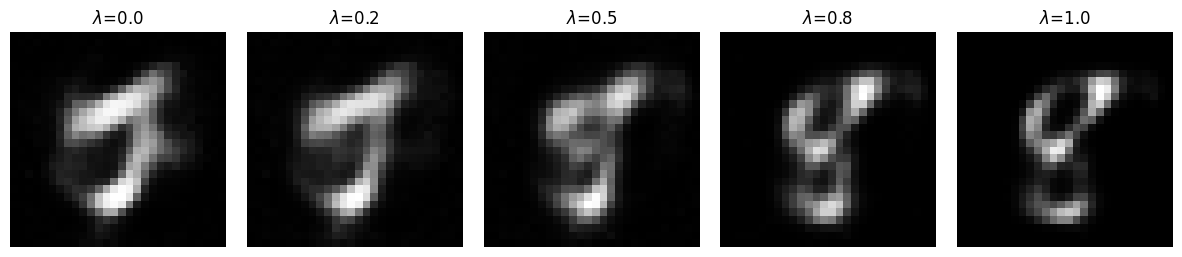
\includegraphics[width=0.8\textwidth]{figures/vae-latent-space.png}
    \caption{Interpolation in VAE latent space}
    \label{fig:vae-latent-space}
\end{figure}
\vspace{-20pt}

\subsubsection{Generation Mechanism}

In GANs, the Generator produces data by mapping a random noise vector $z$ (sampled from a simple prior distribution)
to a data sample $x = G(z; \theta^{(G)})$.
This process is feedforward and data is synthesised without reference to existing inputs.

In VAEs, generation also starts by sampling $z \sim p(z)$.
The decoder $p_\theta(x \mid z)$ then generates a data sample $x$ from the latent variable.
Training also requires the encoder, but generation also relies solely on the decoder and prior.
